\chapter{Methodology}\label{chap:Methodology}

In this section we are going to explain the research idea and introduce the inverse kinematics benchmark environment. Further we will dive a bit deeper into the techniques how to create a dataset and explain the used criterions for the latent models. We are going to conclude this chapter by providing a short introduction into the software written and used tools.

\section{Research Idea}

The primary research idea of my thesis is to pursue a transformation from the RL environment action space $\mathcal{A}$ into a lower-dimensional latent action space $\mathcal{A}_L$. This latent action space will align with the latent space between the encoder and decoder of a VAE model or the feature space of a feed-forward-neural network. By doing so, we aim to enable RL agents to effectively explore and learn within a more compact and smoothened action representation. An schematic drawing can be revisited at \figref{fig:research_idea}

We propose two potential approaches for achieving this reduction in dimensionality: VAEs and supervised models.

In the VAE approach, a conditional or unconditional generative model is employed to learn a latent representation of the action space. By training the VAE on actions from an expert or on state target combinations to emphasis a solution which is independent from an expert, we aim to capture the underlying structure and patterns within the action space from the RL environment. This latent representation can potentially offer a more concise and informative representation of the actions, encourage more efficient learning and exploration for RL agents.

Alternatively, the supervised model approach involves training a supervised learning model, such as a neural network, to directly transform the a defined lower dimensional latent action into the high-dimensional action space. This transformation is learned based on labeled examples of actions and their corresponding latent representations. In the conducted experiments the lower dimensional-action space is just the desired action outcome. By leveraging supervised learning techniques, we aim to find a mapping between state information and desired action outcome to the RL environment action space, allowing RL agent to operate effectively on a higher level within the reduced-dimensional latent action space.
\begin{figure}
	\centering
	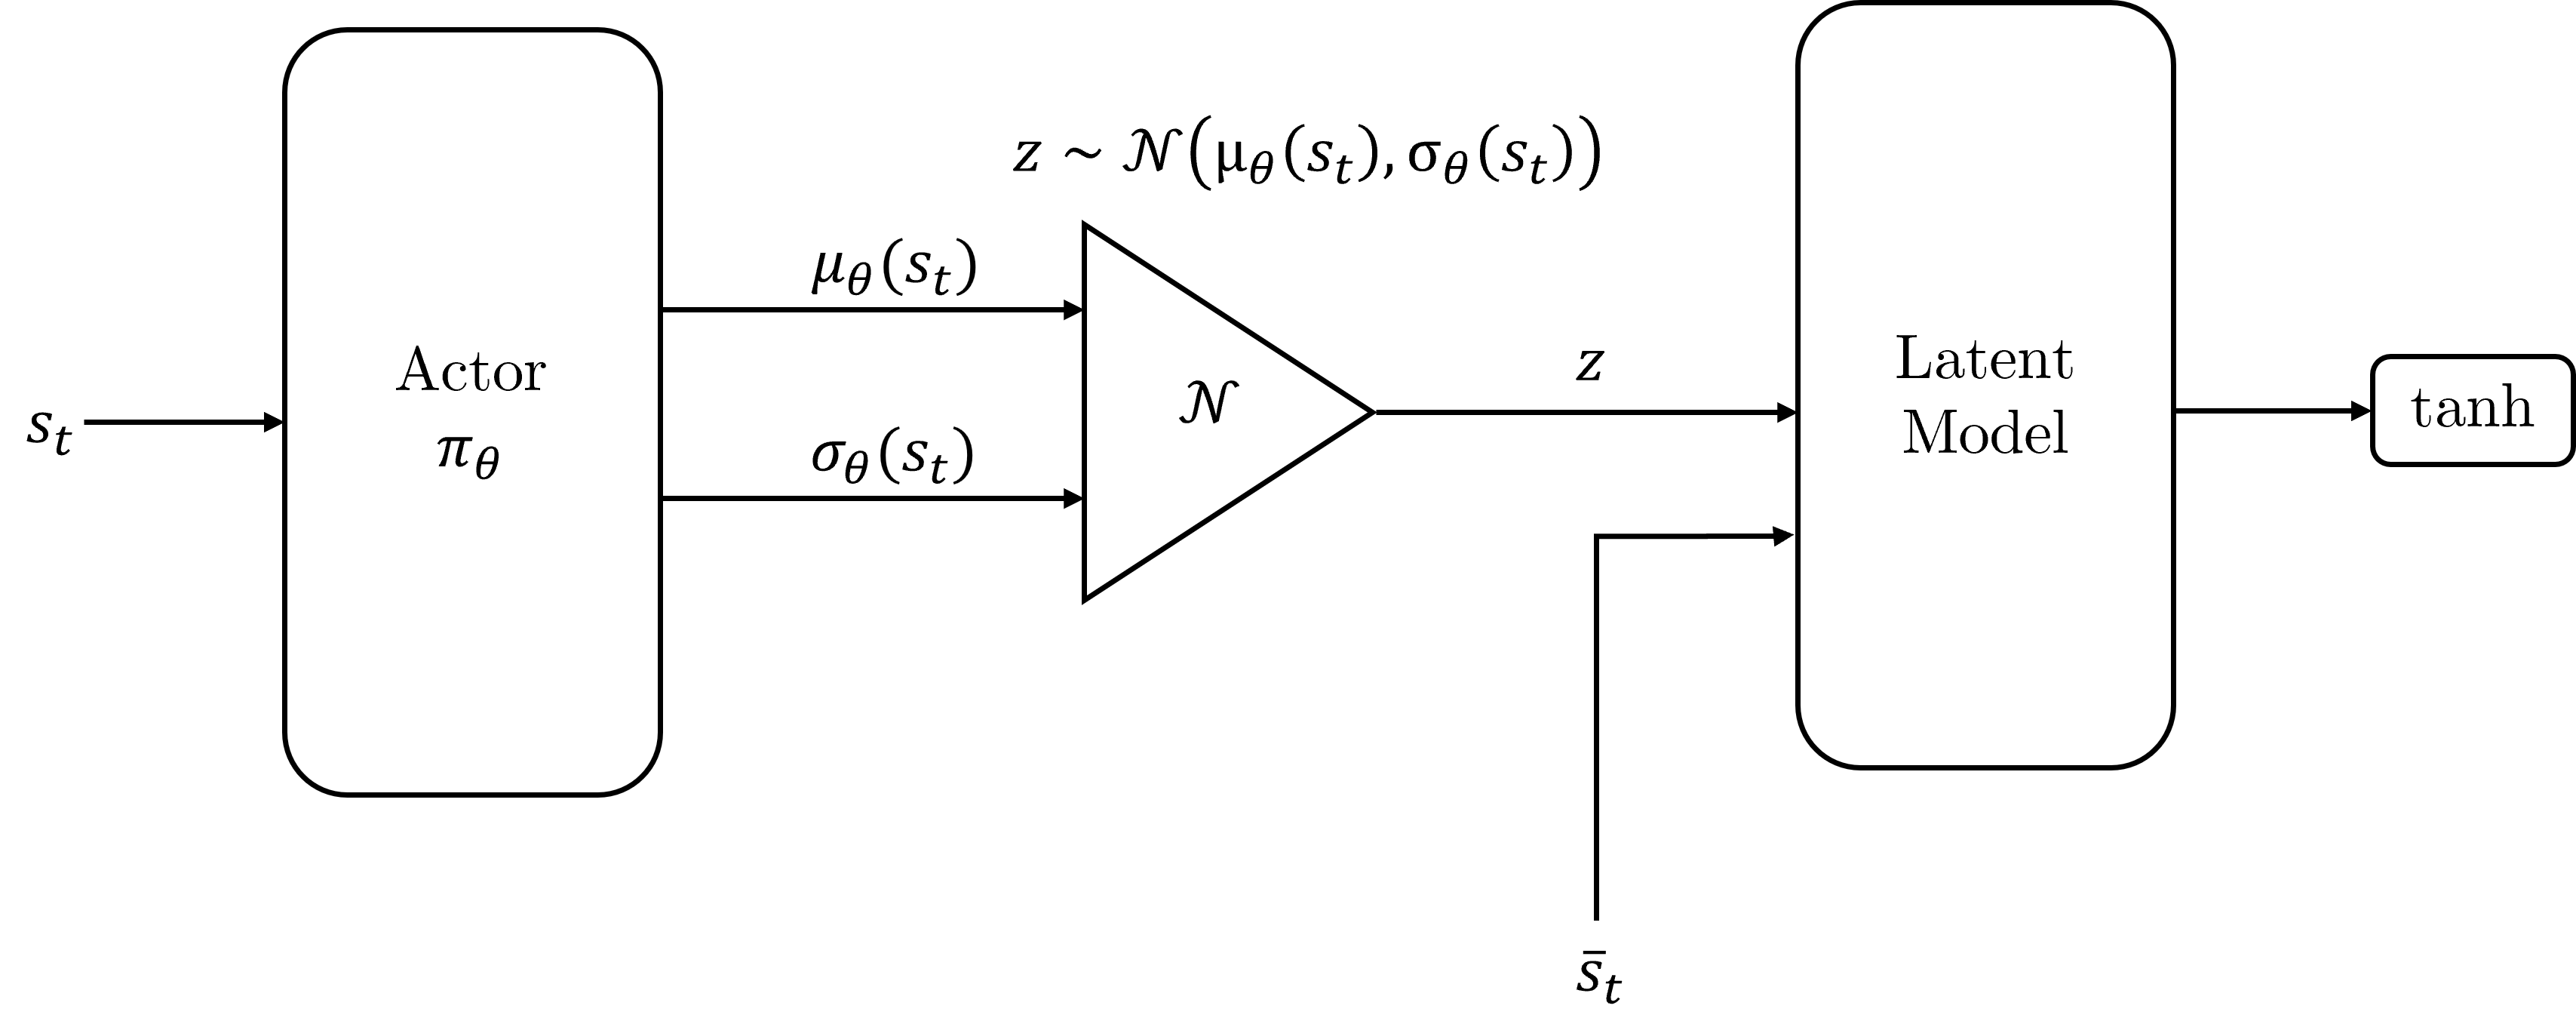
\includegraphics[width=0.7\textwidth,]{figures/methodology/SAC+LatentModel.png}
	\caption[Research idea]{Schematic drawing of how the models would be chained together. The laten model will be replaced by either the decoder of a VAE, a CVAE or a supervised feed forward network. Note that we adapt the additional information $\bar{s_t}$ by the needs of the individual models. }
	\label{fig:research_idea}
\end{figure}

\section{RL Environment}\label{sec:RL-Environment}

To apply RL in general you need an environment the agent can send actions to and receives feedback as discussed in \secref{sec:RL-Framework}. As previously introduced the key problem we are targeting is inverse kinematics of a robot arm. This problem turn out to be suitable because:
\begin{itemize}
    \item the action space is scalable by simply adding additional joints to the robot arm
    \item it can be simplified into a 2D space with a fast and reliable implementation
    \item it is expandable. You are always able to extend the environment with additional constrains like objects the robot has to navigate around or joint angle constrains.
\end{itemize}

In this section we are going to present the a novel RL-Environment for bench-marking the performance of different algorithms to solve inverse kinematics for a robot arm with $N$ many joints and subsequently $N$ many segments with lengths $l \in\mathbb{R}_{>0}^N$ in 2D space. For simplicity reasons $l$ is constant with $l = \{1\}^N$ as a vector with length $N$ and filled with ones. The environment is embedded into the Farama Gymnasium framework~\cite{Gymnasium}.

\begin{figure}[h]
	\centering
	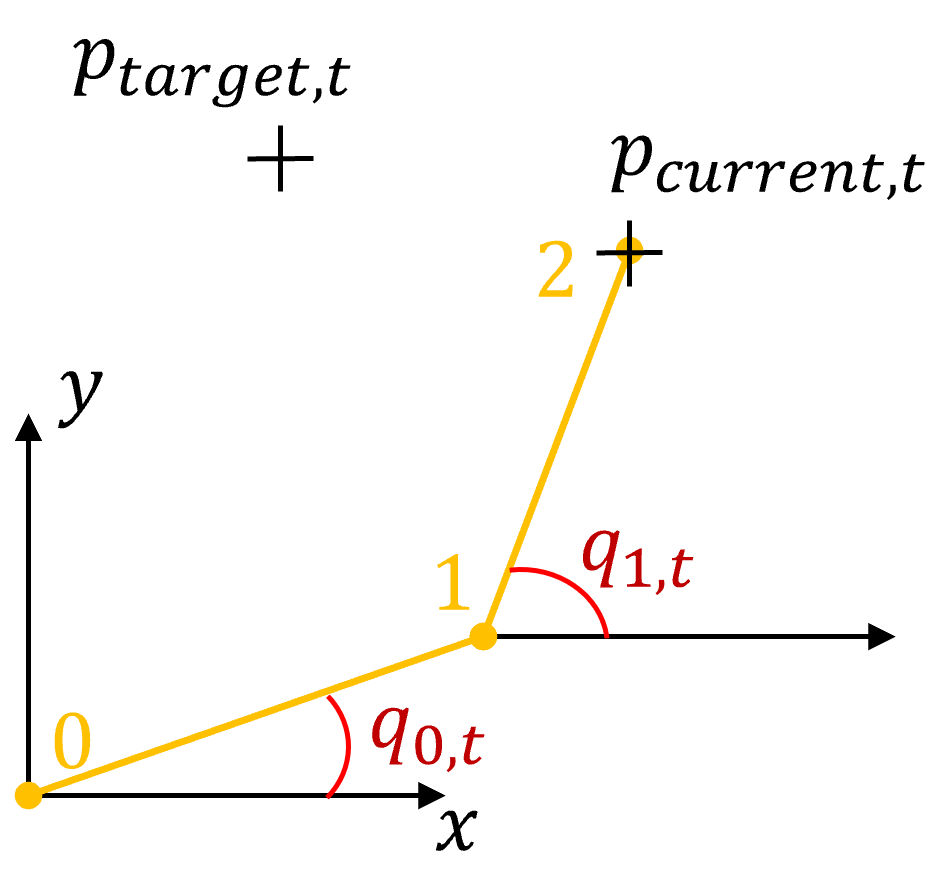
\includegraphics[width=0.4\textwidth,]{figures/methodology/EnvExample.png}
	\caption[Plane Robot Environment]{Schematic drawing of the individual state space components.}
	\label{fig:plane_robot_env}
\end{figure}

\subsection{State Space}

The state space $\mathcal{S} \subset \mathbb{R}^{4 + N}$ for this environment consists of three main building blocks. 

\begin{itemize}
    \item \textbf{goal information} $p_{\text{target}, t} \in \mathbb{R}^2$: This vector provides information where to move the end-effector. This position is lies always in for the robot arm, reachable distance. Mathematical speaking: $||p_\text{target}||_2 \leq \sum_{i = 1}^N l_i$ 
    \item \textbf{state position} $p_{\text{current},t} \in \mathbb{R}^2$: This vector contains the current end-effector position in 2D space and should help the agent to understand where the end-effector is placed and how an action has influenced the current end-effector position. Because the current position is attached to the robot arm: $||p_\text{current}||_2 \leq \sum l$.
    \item \textbf{joint angles} $q_t \in [0, 2\pi^N)$: This vector contains information about the joint angle configuration at time $t$. Note that each joint angles describes the delta angle between the joint direction and a horizontal line from origin in positive x direction.
\end{itemize}
A state $s_t \in \mathcal{S}$ at time $t$ has for all $t$ the same composition

\begin{equation}\label{eqn:state}
    s_t = (p_{\text{target}, t}, p_{\text{current}, t}, q_t)
\end{equation}

To refer to individual parts from index $i$ to $j$ of a state with: $s_{t, (i, j)}$. Therefor we can extract the individual parts with:
\begin{itemize}
    \item $p_{\text{target}, t} = s_{t, (0, 1)}$ 
    \item $p_{\text{current}, t} = s_{t, (2, 3)}$
    \item $q_{t} = s_{t, (4, N + 4)}$
\end{itemize}

\subsection{Action Space}

The action space $\mathcal{A} \subseteq \mathbb{R}^N$ for this particular environment is continuous and contains all possible joint angle configurations for a robot arm with $N$ joints. 

A generated action $\hat{a}$ from the agent is sent to the environment. Inside the environment the incoming action is added on top of the current state angles $q_t$. To ensure the constrains of $q_{t+1} \in [0, 2\pi)^N$ we take the signed remainder of a division by $2\pi$ to write into $q_{t+1}$:
\begin{equation*}
    q_{t+1} = (q_t + \hat{a}) \ \% \ 2\pi
\end{equation*}

Subsequently after updating the state angles the current end-effector position get updated by a forward kinematics call on $q_{t+1}$:
\begin{equation*}
    p_{\text{current}, t} = \text{FK}(q_{t+1})
\end{equation*}


\subsection{Reward Function}

The reward function $R: \mathcal{A} \times \mathcal{S} \to \mathbb{R}$ as in~\eqref{eqn:Rewardfunction} for the conducted experiments and this environment aims to minimize the distance between the current end-effector position $p_{\text{current}, t}$ and the current target position $p_{\text{target}, t}$. The current end-effector position is calculated by the forward-kinematics function on state-angles $q_t$ plus action $a_t$. The target position is sampled at the beginning of an episode and stays constant throughout the episode until completion or time limit is reached. 

\begin{equation}\label{eqn:Rewardfunction}
    R(s_t, a_t) = ||FK(s_{t, (4, \ldots, N + 4)}  + a_t), s_{t, (0 ,1)}||_2
\end{equation}

If you want to normalize the reward function you have to divide $R$ by $N$.

\begin{figure}[h]
	\centering
	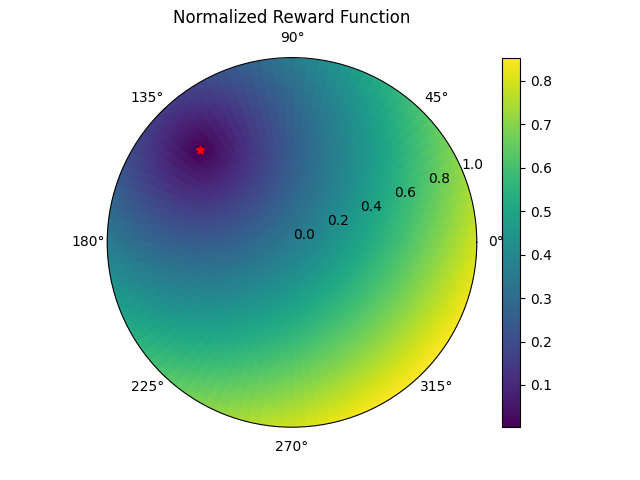
\includegraphics[width=0.5\textwidth,]{figures/methodology/RewardFunction.png}
	\caption[Reward function]{Normalized Reward function with $q \in [0, 2\pi]^N$ as element of the whole space and $p_\text{target} = [-0.5, 0.5]$. The target position $p_\text{target}$ is marked with a red start.}
	\label{fig:Reward_function}
\end{figure}

In \figref{eqn:Rewardfunction} we can see the linear gradient for any current position towards the target position at $[-0.5, 0.5]$.

\section{Dataset Creation}\label{sec:Dataset_creation}

To realize the idea of joining a latent model to the actor network of SAC we do need a dataset to train such latent model. A dataset should contain environment state information as well as possible actions.
Consistent over all experiments with the VAE and Supervised Model sizes of the datasets are consistent:
\begin{itemize}
    \item train: 10.000 data points
    \item validation: 2000 data points
    \item test: 1000 data points
\end{itemize}

\subsection{Uniform Sampling} \label{sec:vanilla_sampling}

The vanilla sampling algorithm for sampling a dataset is to sample state angles $q_t$ and actions $a_t$ from a uniform distribution

\begin{equation} \label{eqn:angle_sample}
    q_t, a_t \sim \mathcal{U}_{[0, 2\pi)}^N
\end{equation}

and the target position with

\begin{align}
    p &= [\cos(\beta), \sin(\beta)] \cdot r \label{eqn:position_sample}\\
    \beta &\sim \mathcal{U}_{[0, 2\pi)} \ \ r \sim \mathcal{U}_{[0, N]} \nonumber
\end{align}

While observing $p_{\text{current}, t}$ in \figref{fig:Uniform_dataset/scatter} we can observe that with an increasing number of joints the scattered dots are forming a two dimensional gaussian distribution around the origin. As we can see in \figref{fig:Uniform_dataset/std} the standard deviation is exponentially decreasing. 
\begin{figure}
    \begin{center}
        \subfloat[Scatter plot of different end effector positions generated by applying forward kinematics on uniformly sampled angles. The end effector positions are normalized by their corresponding number of joints. This leads to the constrain that all positions have a maximum distance to the origin of 1. For each number of joints we sample $5\mathrm{e}{3}$ angles. The upper and right plot are describing the desnsity function of an end-effector position.]{
            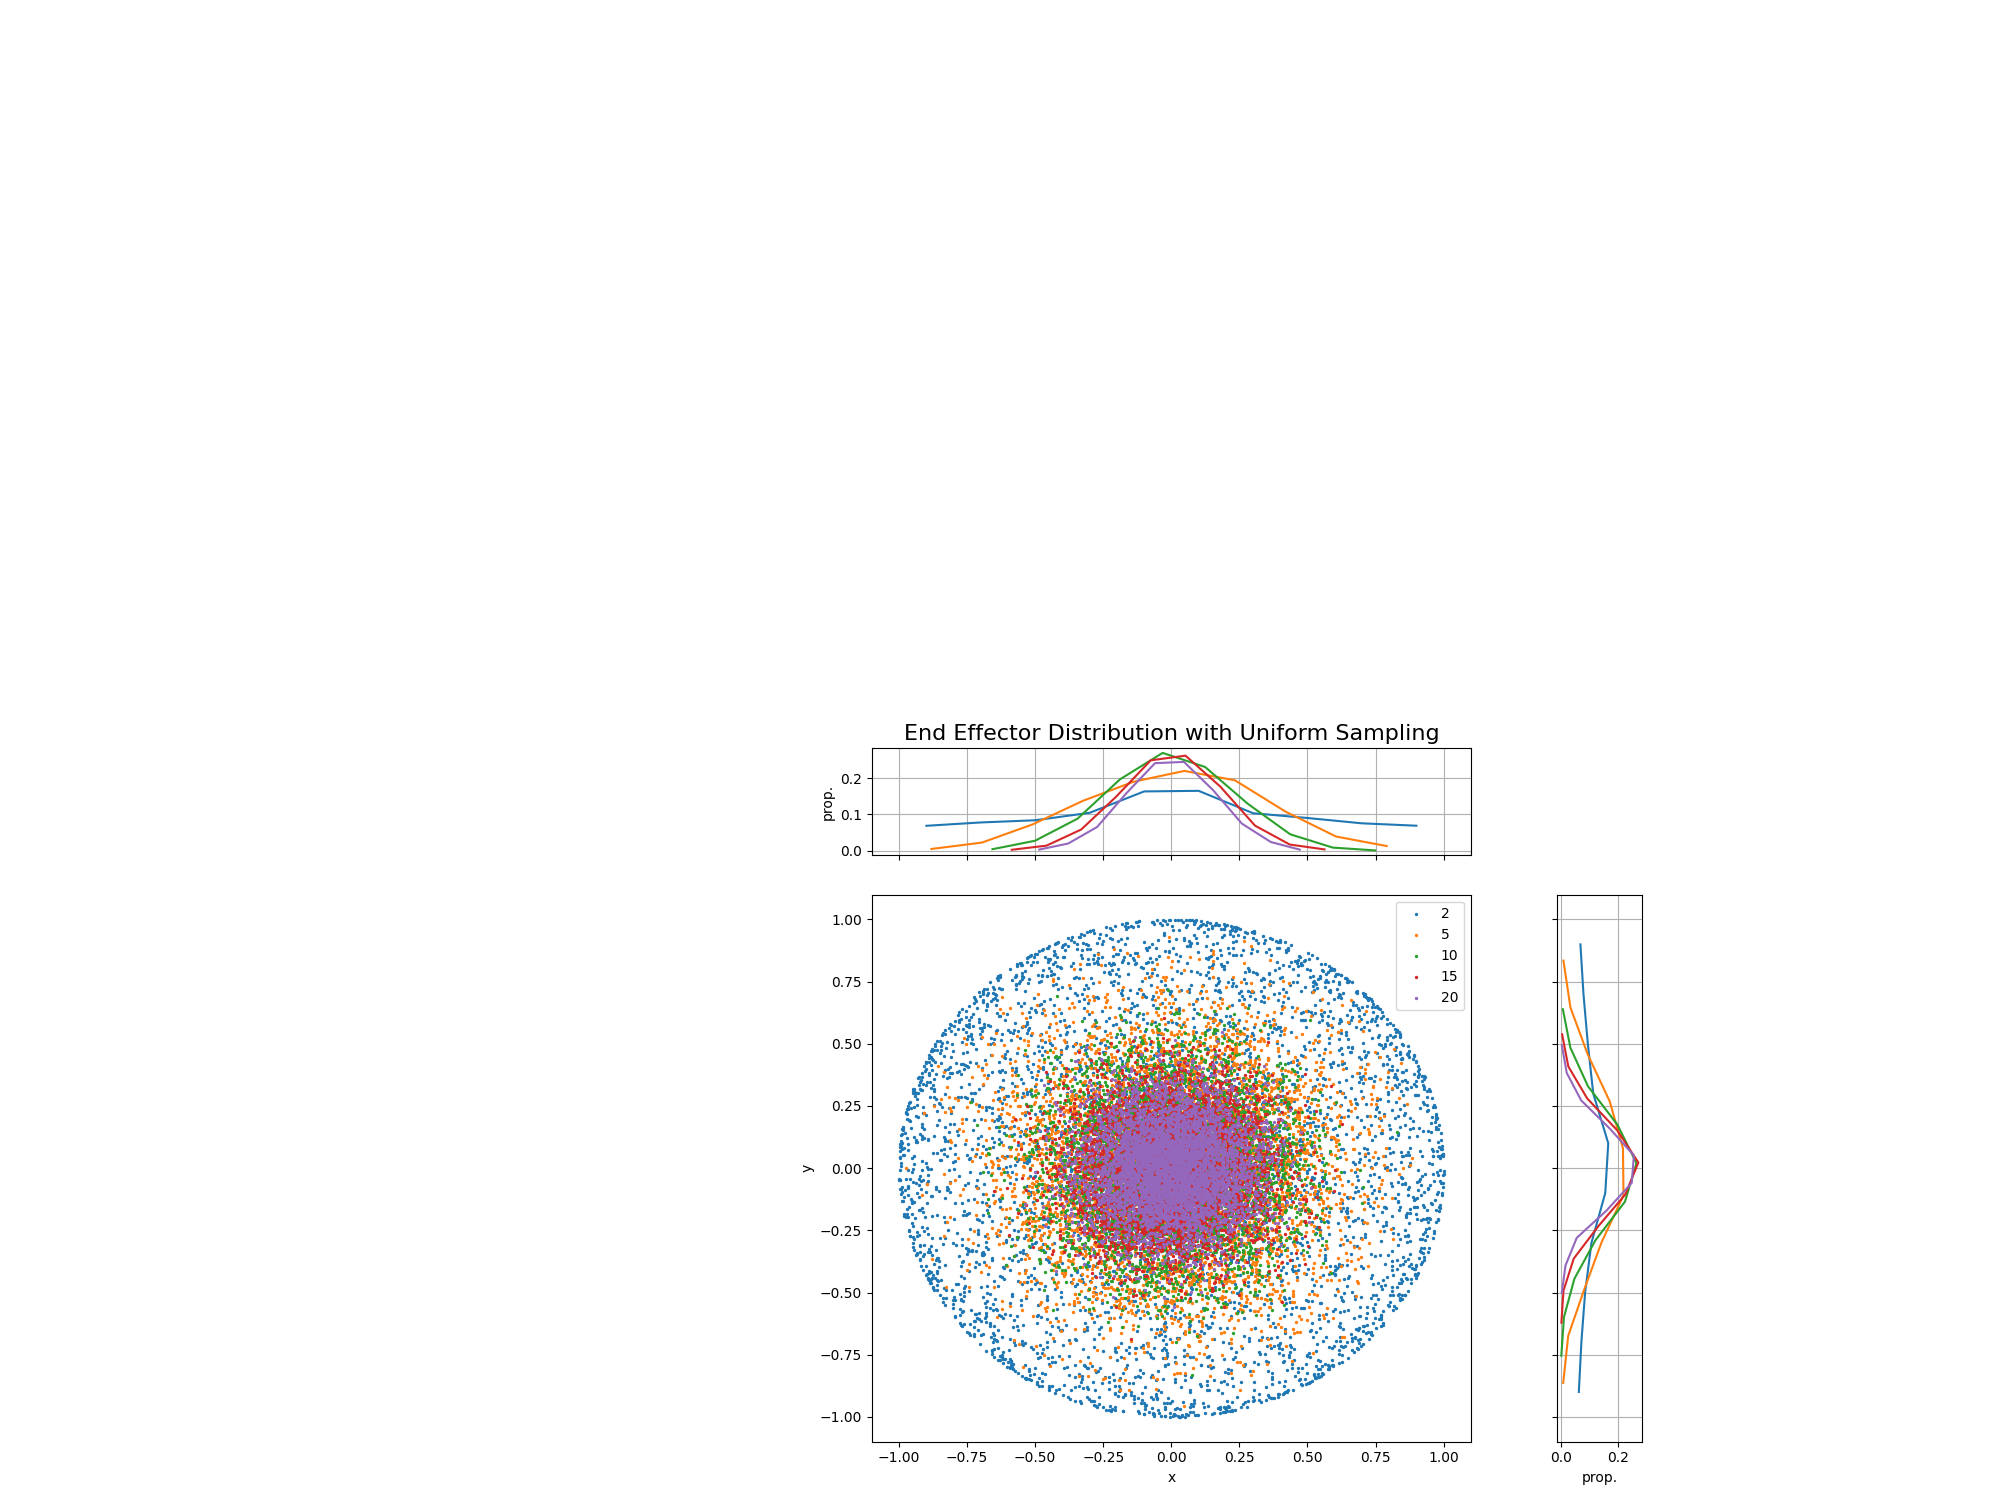
\includegraphics[trim={18cm 0 5cm 3cm}, width=0.46 \linewidth]{figures/methodology/relative_end_effector_scatter.png}\label{fig:Uniform_dataset/scatter}}
        \hfill
        \subfloat[Standard deviation of end effector positions in x and y direction with repsect to the number of joints for a robot arm. For each number of joints we sample $1\mathrm{e}{4}$ angles. ]{
        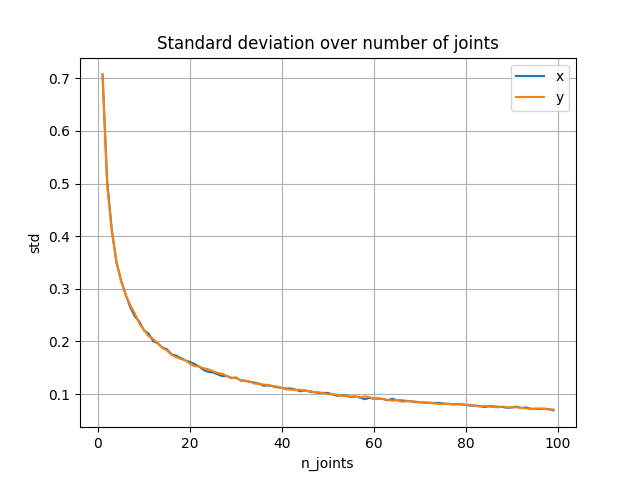
\includegraphics[width=0.46 \linewidth]{figures/methodology/std_over_n_joints.png}\label{fig:Uniform_dataset/std}}
    \end{center}
    \caption[Uniform dataset properties]{Properties of dataset with actions sampled from a uniform distribution. }\label{fig:Uniform_dataset}
\end{figure}

In our application this makes the vanilla algorithm not suitable because we are not covering the observation space close to the maximum reach of the robot arm with more than 2 joints. 

\subsection{Expert Guidance}

The problems encountered with the vanilla sampling algorithm in \secref{sec:vanilla_sampling} lead to the development of an sampling algorithm guided by an expert. 

\begin{algorithm}
    \caption{Expert Guided Dataset Creation}\label{alg:Expert_Dataset}
    \begin{algorithmic}
        \State{} Input: number of joints: $N$, number of samples: $K$.
        \State{} $\mathcal{D} \leftarrow \{\}$  Dataset
        \For{$i \in [0, \ldots, N -1]$}
            \State{} $p_{\text{current}} \leftarrow (\text{\ref{eqn:position_sample}})$ sample a position in 2D space with~\eqref{eqn:position_sample}
            \State{} $q_t \sim \mathcal{U}$ sample initial arm angles from a uniform distribution as in~\eqref{eqn:angle_sample}
            \State{} $q_t \leftarrow IK(q_t, p_{\text{current}})$ solve IK for $p_{\text{current}}$ and with $q_t$ as start
            \State{} $p_{\text{target}} \leftarrow (\text{\ref{eqn:position_sample}})$ sample a position in 2D space with~\eqref{eqn:position_sample}
            \State{} $a_t \leftarrow IK(q_t, p_{\text{target}}) - q_t$ IK for the target position
            \State{} $\mathcal{D}_i \leftarrow ((p_{\text{target}}, p_{\text{current}}, q_t), a_t)$
        \EndFor{}
\end{algorithmic}
\end{algorithm}
The clear advantage from this algorithm is that we ensure now that $p_{\text{target}}$ and $p_{\text{current}}$ are uniform with respect to direction and distance to origin.

On the other hand we are now  bound to the actions the $IK$-solver, in our application CCD as in \algoref{alg:CCD}, is providing. This could lead to unpredicted behavior of the RL agent if we leaf the covered part of $q_t$ as shown in \figref{fig:dataset_action_correlation}. Another disadvantage is that this algorithm is now much slower compared to the vanilla sampling algorithm. 
\begin{figure}
    \begin{center}
        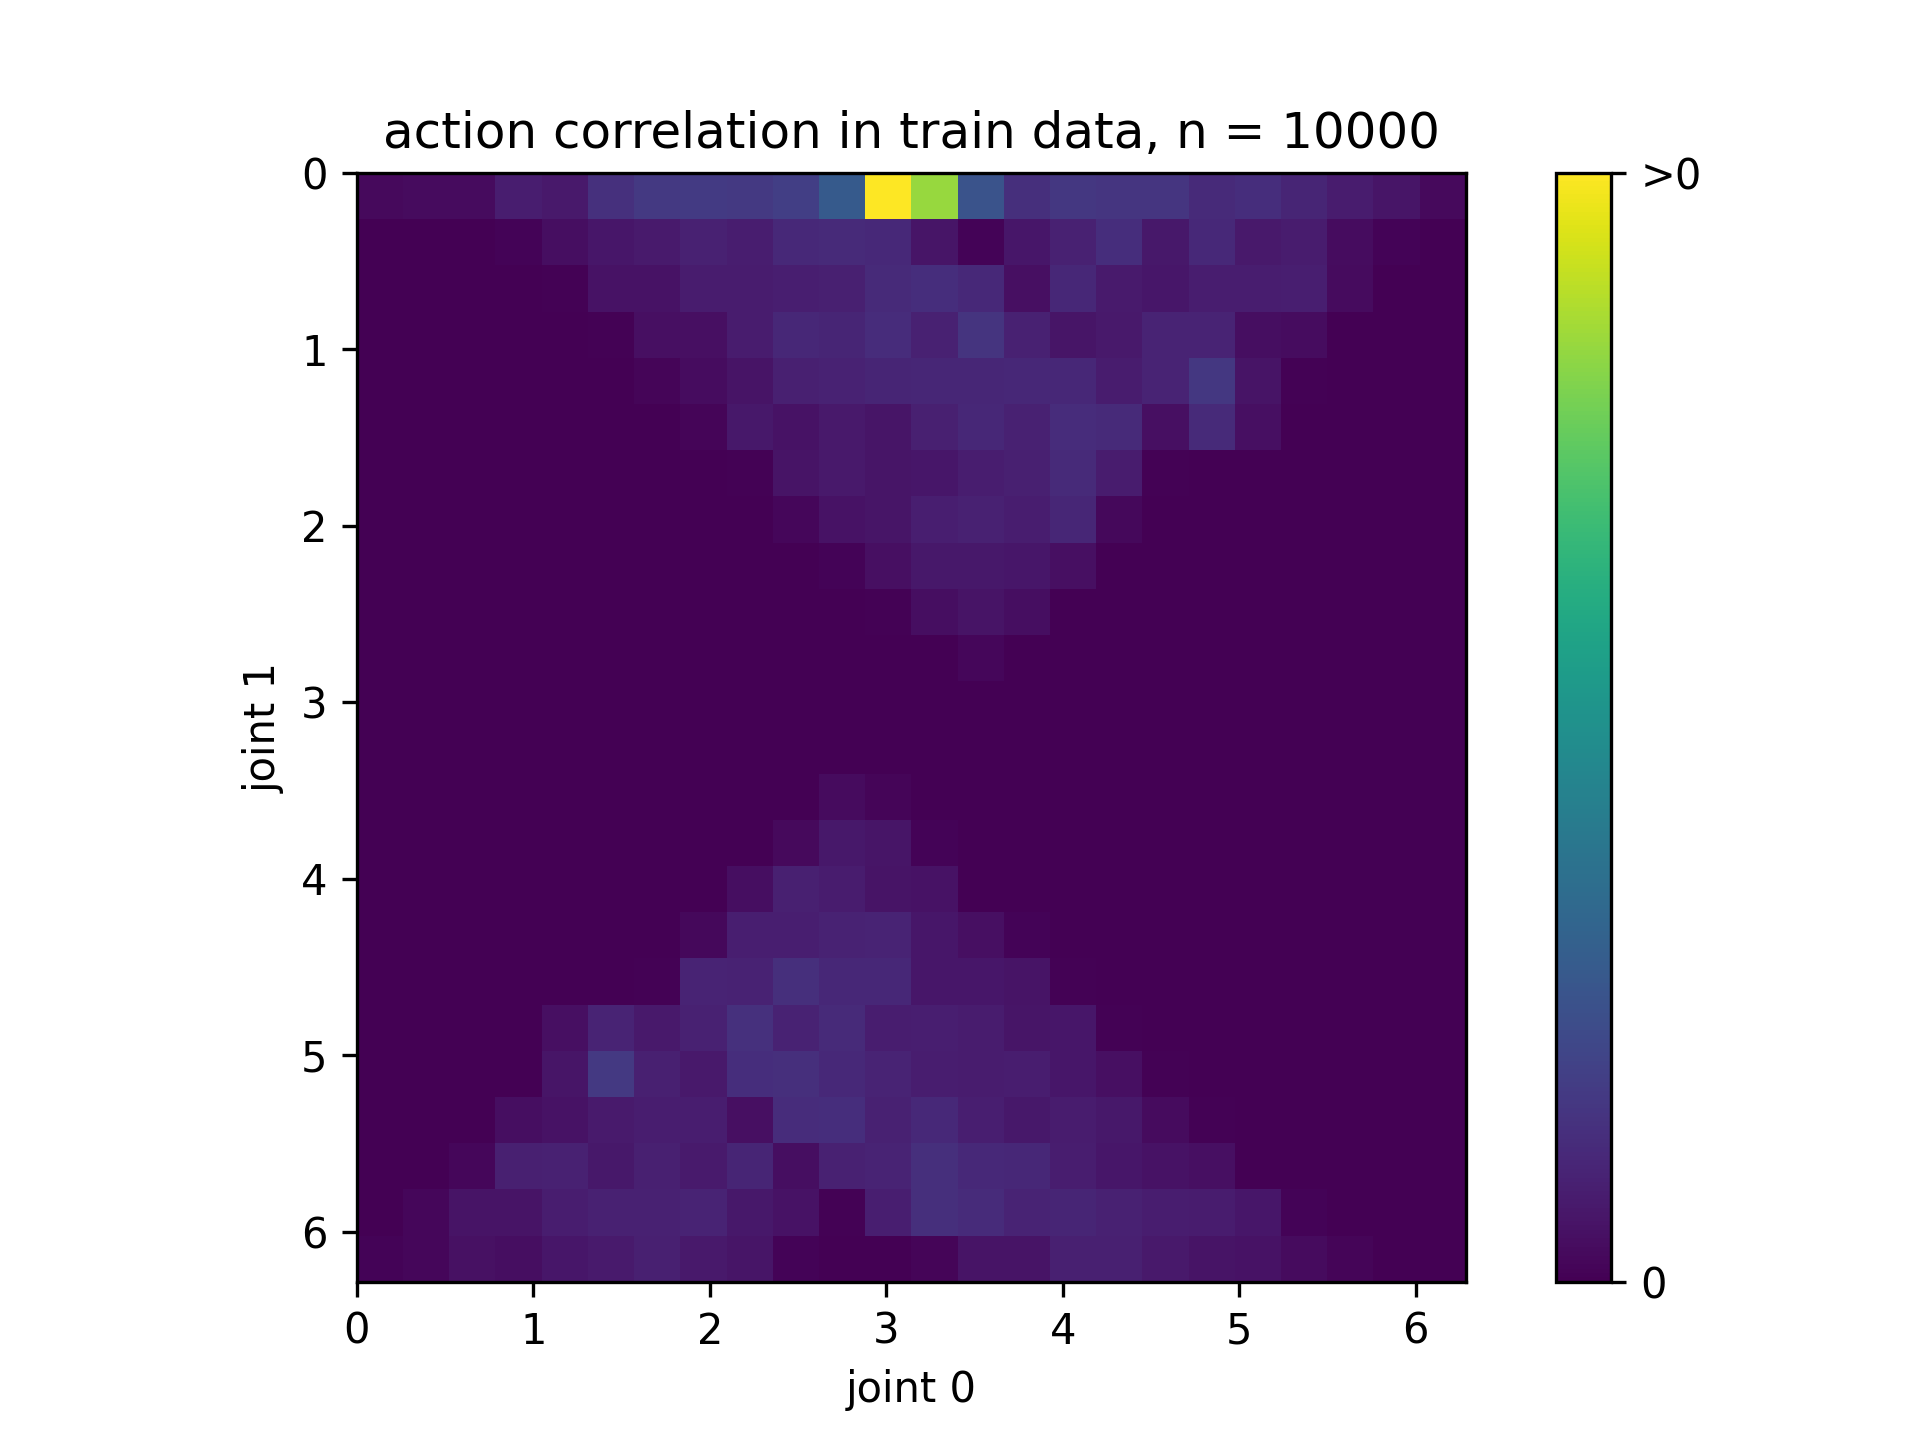
\includegraphics[width=0.46 \linewidth]{figures/methodology/dataset/action_correlation.png}
    \end{center}
    \caption[action correlation CCD]{Plotted is the state angle correlation of two joints as a 2D histogram. Each bucket can be translated to the amount of angles in one 3D bucket $b$ with limits $b_{0, 0}, b_{0, 1}, b_{1, 0}, b_{1, 1}$. Mathematical speaking: $|b| = |\{q_t | q_t \in [0, 2\pi)^2 \land q_{0, t} \in [b_{0, 0}, b_{0, 1}] \land q_{1, t} \in [b_{1, 0}, b_{1, 1}]\}|$}
    \label{fig:dataset_action_correlation}
\end{figure}

To have a more detailed look into the runtime complexity we focus in the runtime complexity of CCD as this is the slowest part of \algoref{alg:Expert_Dataset}. We can observe that the runtime of each CCD run is different since CCD belongs to the family of iterative inverse kinematics solver and the runtime is either limited by a given maximum number of iterations or a break condition depending on how close we are to the goal. \\
In \figref{fig:expert_dataset/runtime_histograms} we can see that all continuous probability density functions have a similar shape but with different standard deviations and means. Since we are interested in the runtime complexity of CCD we plotted the mean runtime of each density function in \figref{fig:expert_dataset/runtime_complexity}. Here we can observe that the runtime complexity of CCD is at least $\mathcal{O}(N^k)$ with $k \geq 3$ since the first order empirical derivation is still at least quadratic. Further derivations would be not plausible because with each derivation we would decrease the number of datapoints by one and therefor having no points left anymore.
\begin{figure}
    \begin{center}
        \subfloat[continuous desnsity function of collected runtimes of ccd over different amount of joints. For each joint we sampled 1000 differnt start conditions, (target, angles) for ccd to solve inverse kinematics. ]{
            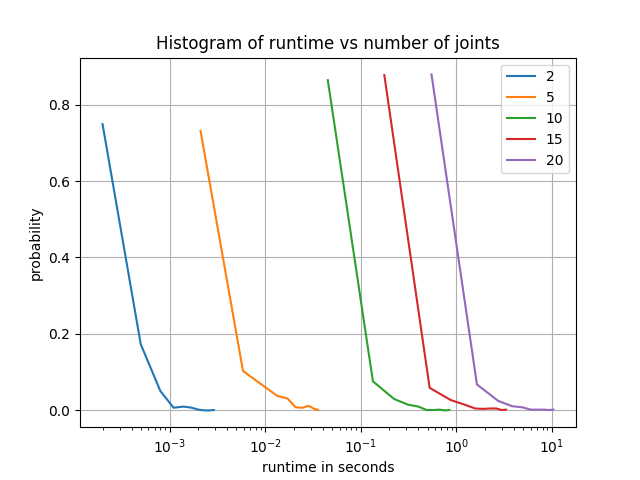
\includegraphics[width=0.46 \linewidth]{figures/methodology/dataset/runtime_histograms.png}
            \label{fig:expert_dataset/runtime_histograms}
            }
        \hfill
        \subfloat[plotted is the mean runtime for 1000 runs of ccd over the number of joints]{
        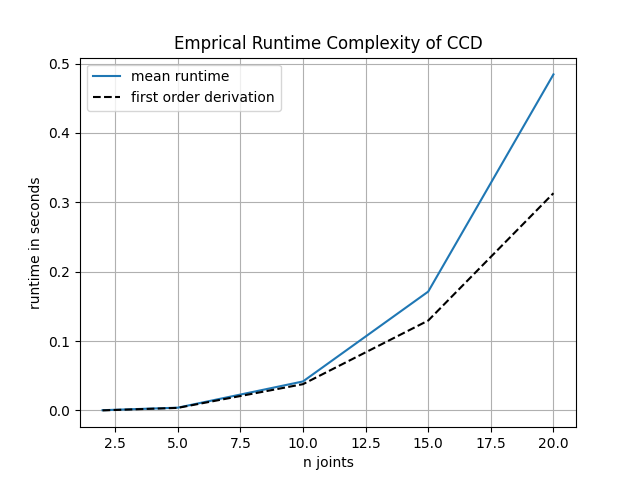
\includegraphics[width=0.46 \linewidth]{figures/methodology/dataset/runtime_complexity.png}
            \label{fig:expert_dataset/runtime_complexity}
            }
    \end{center}
    \caption[Runtime complexity CCD]{Runtime complexity CCD}
    \label{fig:expert_dataset}
\end{figure}

Another interesting point of view is the correlation between resulting angles from ccd. Since we are limited to maximal two dimensional plot we can only plot a heatmap to show the correlations between state joint actions as in \figref{fig:dataset_action_correlation}. Important to note is that the actions are already in environment format and therefor are absolute angles with respect to a horizontal line in positive x direction. We can clearly see that CCD does not use the whole space but only focuses on a rhombus shaped area. 

\section{Latent Criterion}


In this section I will cover the employed loss functions to train the latent models. 
As discussed in \secref{sec:VAE} we employ the Evidence Lower Bound as the objective function to train Variational Autoencoder. To fit our problem of inverse kinematics we tried out 3 different reconstruction loss function.

In this section we will explain the tangible KL divergence as well as the individual reconstruction loss functions.

\subsection{Kulback Leiber Divergence}

The Kulllback Leiber divergence first published by Solomon Kullback and Richard Leiber  in 1951~\cite{pml2Book} is mathematical measure of how a probability distribution $P$ differs from a second distribution $P'$ and is denoted as $D_\text{KL}(P||P')$. Inside the ELBO it functions as a regularization element between the latent distribution $p_\phi(z|x)$ and a target distribution $p(z)$. Throughout this thesis we take the standard normal distribution as the target distribution, $p(z) = \mathcal{N}(0, I)$. Since we implement a parameterized gaussian as the latent distribution due to the nature of continuous input data, $p_\phi(z|x) = \mathcal{N}_\phi(\mu_\phi(x)| \ \Sigma_\phi(x))$. Therefor we can calculate the Kullback Leiber Divergence as:
\begin{align*}
    D_\text{KL}( \mathcal{N}_\phi(\mu_\phi(x)| \Sigma_\phi(x))|| \mathcal{N}(0, I)) &= \frac{1}{2} \left(\mu_\phi(x)^T\mu_\phi(x)  + tr\left(\Sigma_\phi(x)\right) - K - \log{|\Sigma_\phi(x)|} \right)\\
    &= \frac{1}{2} \left(\mu_\phi(x)^T\mu_\phi(x)  + \sum_{i=1}^K\Sigma_\phi(x)_{ii} - K - \log\left(\sum_{i=1}^K\Sigma_\phi(x)_{ii}\right)\right) 
\end{align*}

\subsection{Reconstruction Loss}

Inside the Evidence Lower Bound objective, the reconstruction loss minimizes the distance between the input data $x$ and the model output $\hat{x}$. In our experiments we employed three different approaches for the reconstruction loss:

\textbf{Imitation Loss}. The imitation loss is a criterion to minimize the mean squared error between a given label $y$, in this case an action from an expert which results in $y \in \mathbb{R}^N$ and the predicted action $\hat{x} \in \mathbb{R}^N$. It is defined as in~\eqref{eqn:Imitation-Loss}.

\begin{equation}\label{eqn:Imitation-Loss}
    \begin{split}
        \mathcal{L}_\text{Imi}: \mathbb{R}^N \times \mathbb{R}^N & \to \mathbb{R} \\
        y, \hat{x} & \mapsto \frac{1}{N}\sum_{i = 0}^{N-1} \left(y_i - \hat{x}_i\right)^2 
    \end{split}
\end{equation}

\textbf{Distance Loss}. This loss function minimizes the distance between a desired position in 2D space as label $p_\text{target}$ and the action outcome of a state action combination. The state information needed for this criterion are only the current robot arm angles $q$. Like before the action is referred to as $\hat{x}$.

\begin{equation}\label{eqn:Distance-Loss}
    \begin{split}
        \mathcal{L}_\text{Dist}: \mathbb{R}^2 \times \mathbb{R}^2 \times \mathbb{R}^N & \to \mathbb{R} \\
        p_\text{target}, \hat{x}, q & \mapsto ||p_\text{target} - \text{FK}(q + \hat{x})||_2
    \end{split}
\end{equation}

This criterion is also used in a standard supervised learning approach where the model predicts actions based on state information.

\textbf{Inverse kinematics Loss}. This criterion as in~\eqref{eqn:IK-Loss} is the result of merging distance loss and imitation loss in one loss function as a weighted sum of those two components with weights $w_\text{Imi}, w_\text{Dist} \in \mathbb{R}$. Inside the code, the loss function can be configured to work also a pure distance loss function without providing any expert action and make it therefor also applicable to the afore mentioned supervised learning approach. 

\begin{equation}\label{eqn:IK-Loss}
    \begin{split}
        \mathcal{L}_\text{IK}: \mathbb{R}^2 \times \mathbb{R}^2 \times \mathbb{R}^N, \mathbb{R}^N & \to \mathbb{R} \\
        p_\text{target}, \hat{x}, q, y  &\mapsto w_\text{Imi} \cdot \mathcal{L}_\text{Imi}(y, \hat{x}) + w_\text{Dist} \cdot \mathcal{L}_\text{Dist}(p_\text{target}, \hat{x}, q)
    \end{split}
\end{equation}

\section{Learning the Latent Model}

For the upcoming experiments we settled one setting with one kind of dataset, the TargetGaussian. \\
The idea behind the gaussian target dataset is to learn an action which moves the end-effector towards a target sampled from a two dimensional gaussian distribution around the end-effector as demonstrated in \figref{fig:TargetGaussian_Schematics}.
\begin{figure}
    \begin{center}
        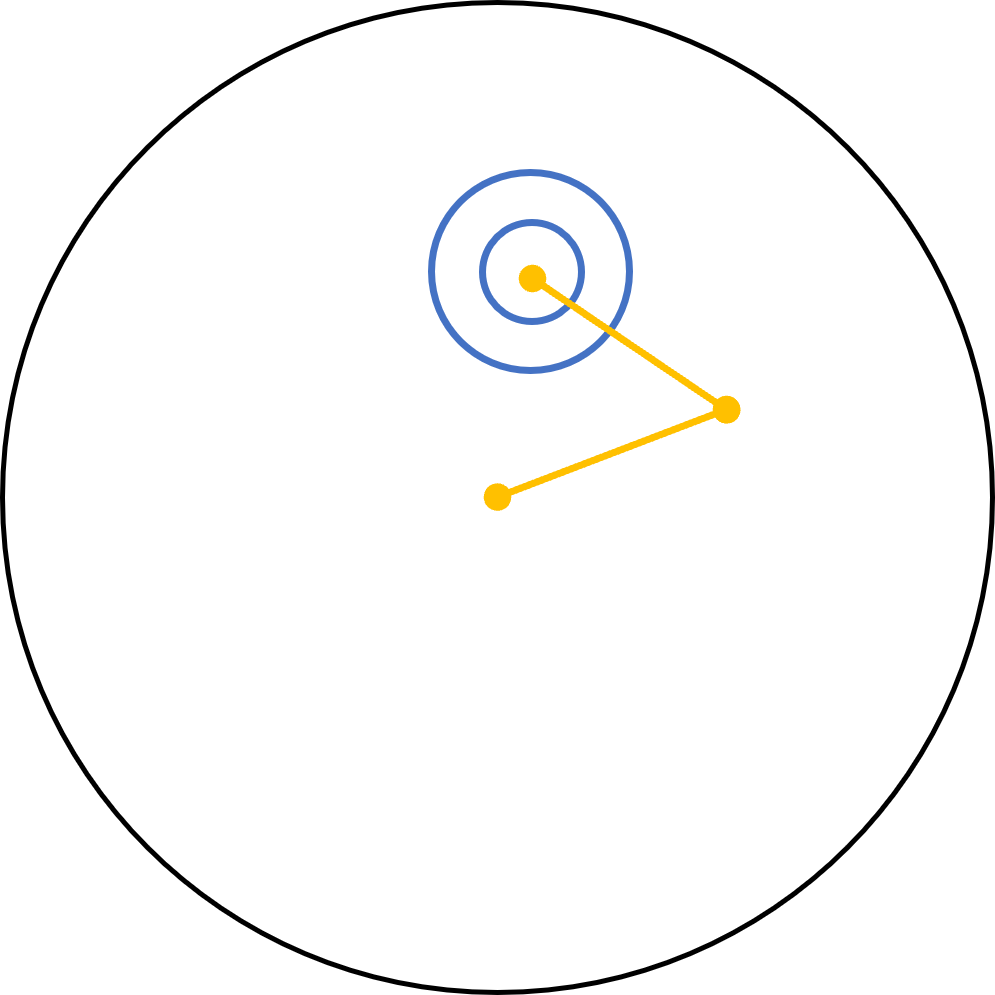
\includegraphics[width=0.3 \linewidth]{figures/experiments/VAE/TargetGaussian.png}
    \end{center}
    \caption[Target Gaussian Schematics]{Schematic drawing how the target gaussian dataset works. First we are going to take the state as is comes form \algoref{alg:Expert_Dataset} (in yellow). Then we are going to sample a target position from inside a the two dimensional truncated or non truncated gaussian distribution (in blue) and define it as new target position. Optionally we can also compute the corresponding CCD action.}\label{fig:TargetGaussian_Schematics}
\end{figure}

\begin{table}[]
    \centering
    \begin{tabular}{l|l}
        Name & Value \\
        \hline
        VAE $x$ & $p_{\text{target}, t}$ \\
        Supervised $x$ & $s_t$ \\
        $c$ & $(p_{\text{current}, t}, q_t)$ \\
        $\hat{x}$ & $q_{t + 1}$
    \end{tabular}
    \caption[Latent workflow parameter]{Latent workflow parameter with their correlation}
    \label{tab:Latent Parameter}
\end{table}

While training the Variational Autoencoder we settled on hyperparameter as described in \chapref{chap:appendix} and input vectors as in \tabref{tab:VAE_parameter}. It is important to note that $x$ for VAE, concatenated with $c$ equal to $s_t$ is which is the same input as for the Supervised model. 

While training VAE and Supervised model you have to account the additional hyperbolic tangent function in the back of \figref{fig:research_idea}. This additional stage in introduced with an instance of \texttt{PosProcessor}. The \texttt{PosProcessor} is enabled during training the latent model but deactivated during training SAC, because SAC applies a hyperbolic tangent function in the \texttt{PolicyNet}. 

\section{Software}

In the following section we are going to present the developed software stack to train the latent models as well as the reinforcement learning agent.

\subsection{Inverse kinematics Environment}

As presented previously in \secref{sec:RL-Environment} we tackle the problem of inverse kinematics of a robot arm with $N$ many joints in a two dimensional setting. 
The implemented environment

\subsection{Latent Module}

The latent module contains every functionality regarding either a Variational Autoencoder or a simple feed forward supervised regression model.
As a deep learning library we build on pytorch 1.\todo{find out version}. 

You can find out about the functionality either with 



\subsection{Soft actor critc}
